\section{Aplikasi "HELLO WORLD"}
Hello World adalah sintax atau script untuk mengetahui aturan sebuah tools tersebut, dimana perintah ini adalah teks yang selalu digunakan dalam pengujian awal suatu program untuk menampilkan output.

\subsection{Nama-nama yang sudah didefinisikan oleh CodeIgniter3}
Hal yang perlu diperhatikan dalam menentukan nama (baik nama controller, fungsi,variabel,maupun konstanta) kita tidak boleh menggunakan nama-nama yang sudah didefiniskan oleh CodeIgniter.

\section{Nama-nama Variabel}
Untuk mendefinisikan variabel, Anda seharusnya tidak menggunakan nama berikut :
\begin{enumerate}
\item \$config
\item \$db
\item \$lang
\end{enumerate}

\section{Controller}
controller adalah sebuah file class yang berujuan dapat berhubungan dengan sebuah URI.
\subsection{Nama-nama Controller}
Berikut ini daftar nama yang tidak dapat Anda gunakan untuk mendefinisikan nama \textit{Controller}
\begin{enumerate}
\item ci\_controller
\item  Default
\item Index
\end{enumerate}

mari coba membuat controller sederhana untuk dapat melihat bagaimana controller bekerja. buat file dengan nama hello.php, dan isikan code seperti dibawah ini.
Dalam tulisan saya sebelumnya adalah tutorial instalasi codeigniter, sekarang kita lanjut ke cara menampilkan Hello World pada CodeIgniter, kenapa hello world?

Disini kita akan menggunakan \textit{Controller} sebagai komponen utama yang memproses permintaan user.
untuk memulainya, kita dapat menjalankan aplikasi Text Editor yang dimiliki. 
lalu kita bisa menuliskan kode, disini ada 2 perintah yang akan saya masukan yaitu untuk perintah lengkap dan perintah \textit{simplenya} tersebut seperti ini:

\begin{figure}[ht]
\center{\includegraphics[width=1.0\textwidth]{figures/HW.jpg}}
\caption{Perintah Hello World Perintah Lengkap}
\label{Gambar 4}
\end{figure}

\begin{figure}[ht]
\center{\includegraphics[width=1.0\textwidth]{figures/HW2.jpg}}
\caption{Perintah Hello World Perintah Simple}
\label{Gambar 5}
\end{figure}

Kita hanya tinggal memilih yang mana yang akan kita masukan dari kedua perintah diatas pada gambar tersebut kemudian simpan file dengan nama hello.php dan ditempatkan di dalam direktori \ref{lst:location}

\verb
C:\XAMPP\htdocs\ci310\application\controllers\\
setelah disimpan, kita dapat menjalankan controller diatas dengan menuliskan url berikut :
http://localhost/ci310/index.php/hello
permintaan diatas akan mengeksekusi metode index() yang terdapat didalam kelas Hello. 
hasil yang diperoleh akan seperti ini :

\begin{figure}[ht]
\center{\includegraphics[width=1.0\textwidth]{figures/HWresult.jpg}}
\caption{Hasil}
\label{Gambar 6}
\end{figure}

\subsection {View}
Proses yang menampilkan hasil output dari suatu model.
Cara membuat view pada codeigniter yaitu pada gambar dibawah ini :
\begin{figure}[ht]
\center\includegraphics[width=1.0\textwidth]{figures/views.jpg}
\caption{Membuat views}
\label{Gambar 7}
\end{figure}
Seetelah membuat kode program seperti gambar diatas simpan \textit{file} diatas dengan nama yang bebas sesuai keinginan masing-masing (misalnya:belajarview.php) dan tempatkan pada direktori berikut \ref{lst:location} :

\verb 
C:\XAMPP\htdocs\ci310\application\views\\
seperti pada gambar dibawah ini :
\begin{figure}[ht]
\center{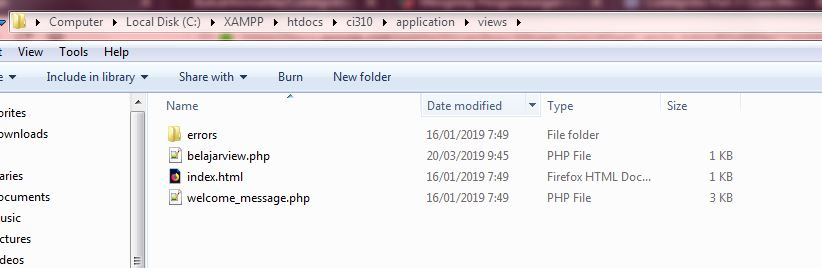
\includegraphics[width=1.0\textwidth]{figures/views1.jpg}}
\caption{Menyimpan Direktori View}
\label{Gambar 8}
\end{figure}
Selanjutnya,kita  harus mengubah file \textit{Controller}

\verb 
application\controllers\hello.php\\

dan hasilnya akan menjadi seperti gambar dibawah ini :
\begin{figure}[ht]
\center{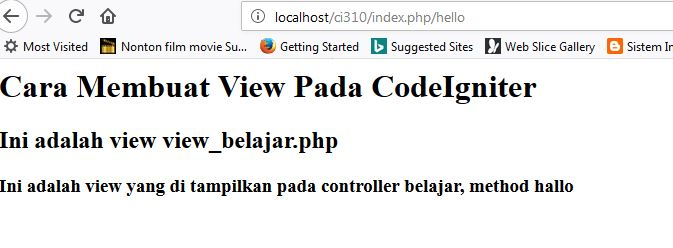
\includegraphics[width=1.0\textwidth]{figures/views2.jpg}}
\caption{Hasil dari View}
\label{Gambar 9}
\end{figure}


\section{Model}
Model biasanya digunakan untuk repsentasi dari struktur data yang terdapat pada CodeIgniter.
Aplikasi juga dapat dibuat hanya dengan menggunakan komponen \textit{controller} dan \textit{model}
tanpa view, meskipun pada praktiknya hal ini seharusnya tidak dilakukan. untuk membuktikannya, 
kita dapat membuat \textit{model} (misalnya dengan nama Hello\_model) 
menggunakan kode berikut :

\begin{figure}[ht]
\center{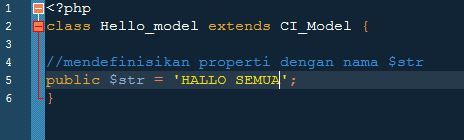
\includegraphics[width=1.0\textwidth]{figures/Model.jpg}}
\caption{Membuat model}
\label{Gambar 10}
\end{figure}
jangan lupa setelah itu kita simpan pada direktori
\verb 
C:\XAMPP\htdocs\ci310\application\models\\

\begin{figure}[ht]
\center{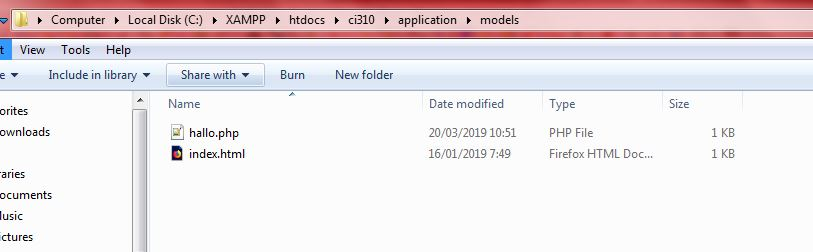
\includegraphics[width=1.0\textwidth]{figures/Model2.jpg}}
\caption{Menyimpan model}
\label{Gambar 11}
\end{figure}

Selanjutnya,kita  harus mengubah file \textit{Controller}

\verb 
application\controllers\hello.php\\
seperti pada gambar dibawah ini :
\begin{figure}
\center{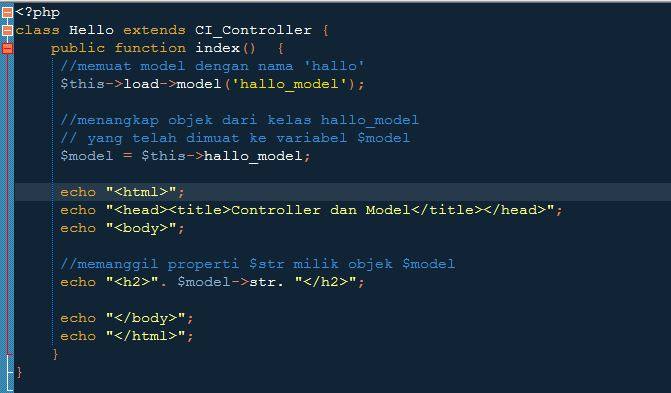
\includegraphics[width=1.0\textwidth]{figures/Model3.jpg}}
\caption{Mengubah model ke controllerl}
\label{Gambar 12}
\end{figure}

dan setelah itu perintah akan dieksekusi dan hasilnya akan seperti ini :

\begin{figure}
\center{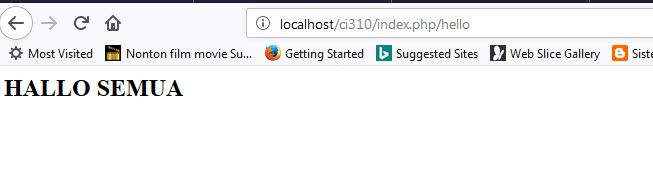
\includegraphics[width=1.0\textwidth]{figures/Model4.jpg}}
\caption{Mengubah model ke controllerl}
\label{Gambar 13}
\end{figure}


\section{Menggunakan Controller,Model dan View}
Aplikasi dengan komponen \textit{Controller, model,view} merupakan aplikasi yang lengkap. pada praktiknya, teknik inilah yang pada umumnya digunakan oleh aplikasi yang dikembangkan menggunakan CodeIgniter.
untuk itu kita akan mencoba mendemonstrasikan dengan melibatkan file ketiga komponen utama ini yaitu\ref{lst:hello}
\begin{figure}
\center{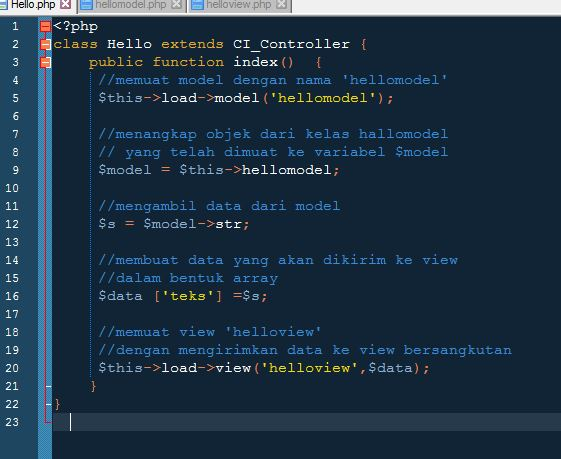
\includegraphics[width=1.0\textwidth]{figures/Hello.jpg}}
\caption{Controller Hellol}
\label{Gambar 14}
\end{figure}

Kemudian masukan perintah file model

\begin{figure}
\center{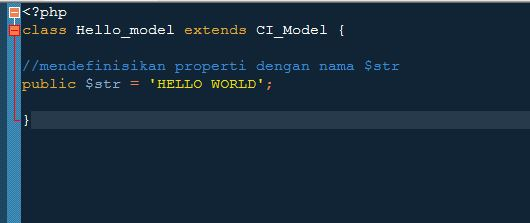
\includegraphics[width=1.0\textwidth]{figures/HelloModel.jpg}}
\caption{Model Hellol}
\label{Gambar 15}
\end{figure}

dan terakhir perintah untuk view

\begin{figure}
\center{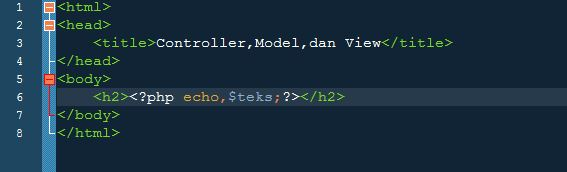
\includegraphics[width=1.0\textwidth]{figures/HelloView.jpg}}
\caption{View Hellol}
\label{Gambar 16}
\end{figure}

Maka untuk hasil akhirnya akan seperti ini :
\begin{figure}
\center{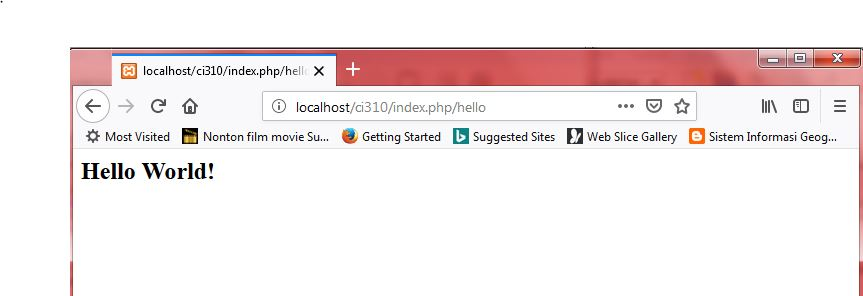
\includegraphics[width=1.0\textwidth]{figures/Result2.jpg}}
\caption{Akhir}
\label{Gambar 17}
\end{figure}



